\begin{minipage}{0.4\textwidth}
{\bf Внешняя задача Дирихле}
% Затехал: Цветкова Ольга
Найти $u(x) \in C^2(\Omega) \cap C(\Omega \cup \Gamma)$, удовлетворяющую условиям:
\[
\begin{cases}
\Delta u(x) = 0, & \Forall x \in \Omega, \\
\eval{u}_{\Gamma} = u_0(x), & x \in \Gamma, \\
u(x) \rightarrow_{|x|\rightarrow \infty} 0.
\end{cases}
\]

Такое решение называется {\bf классическим}.

\end{minipage}
\hfill
\begin{minipage}{0.4\textwidth}
{\bf Внешнаяя задача Неймана}

Найти $u(x) \in C^2(\Omega) \cap C(\Omega \cup \Gamma)$, удовлетворяющую условиям:
\[
\begin{cases}
\Delta u(x) = 0, & \Forall x \in \Omega, \\
\cfrac{\partial v}{\partial \vec n}\bigg|_{\Gamma} = u_1(x), & x \in \Gamma, \\
u(x) \rightarrow_{|x|\rightarrow \infty} 0.
\end{cases}
\]

Такое решение называется {\bf классическим}.

\end{minipage}




Отличие постановок внешних и внутренних задач -- $u(x) \rightarrow 0$ во внешних задачах. Для внутренней задачи Неймана -- даже при выполнении условий разрешимости $\oint u_1(x) dS_x = 0$ решение не единственно.

\begin{theorem}
Не может существовать более 1 классического решения внешней задачи Дирихле.
\end{theorem}
\begin{proof}
Если $u_1,\  u_2$ -- классические решения, то $v(x) = u_1 - u_2$ удовлетворяет полностью однородной задаче 
\[
\begin{cases}
v(x)|_{\Gamma} = 0,\\
v(x) \rightarrow_{|x|\rightarrow \infty} 0 \ (\forall \eps > 0 \Exists \widetilde{R}(\eps)\colon \Forall x \colon |x| > \widetilde{R}(\eps) \rightarrow |v(x)|<\eps).
\end{cases}
\]

\begin{center}
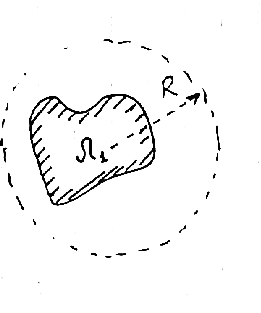
\includegraphics[scale = 0.4]{25_1_new}
\end{center}

Строим сферу радиуса $R \geqslant \widetilde{R}(\eps), \, \Omega_1 \subset B_R(0)$.
По следствию из принципа максимума $|v(x)|\leqslant~\max\limits_{\partial\Omega_1 \cup \partial B_R(0)} |v(y)|\leqslant ~\eps$.

Т.к. $\eps > 0$ было выбрано произвольно, имеем $v(x) \equiv 0 \text{ в } \Omega \cup \Gamma$.
\end{proof}

\begin{theorem}
Не может существовать более 1 классического решения внешней задачи Неймана.
\end{theorem}
\begin{proof}
Если $u_1,\  u_2$ -- классические решения, то $\underbrace{v(x) = u_1 - u_2}_{\text{гармоническая в }\Omega\text{ и }C^2(\Omega)\cap C(\Omega \cup \Gamma)}$ удовлетворяет полностью однородной задаче 
\[
\begin{cases}
\cfrac{\partial v}{\partial \vec n}\bigg|_{\Gamma} = 0,\\
v(x) \rightarrow_{|x|\rightarrow \infty} 0 \ (\forall \eps > 0 \Exists \widetilde{R}(\eps) \colon \Forall x : |x| > \widetilde{R}(\eps) \rightarrow |v(x)|<\eps).
\end{cases}
\]
\begin{center}
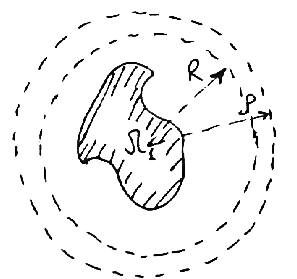
\includegraphics[scale = 0.4]{25_2_new}
\end{center}

Возьмем $R:\ \Omega_1 \subset B_R(0),\ \rho > R$. По 1-й ф-ле Грина для $v(x)$:
\[
\cancelto{0}{\int\limits_{B_R(0) \backslash \Omega_1} \Delta v(x) \cdot v(x) \cdot dx} = 
\cancelto{0}{\oint\limits_{\Gamma} \cfrac{\partial v}{\partial \vec n}(x) \cdot v(x) dS_x} + \oint\limits_{\partial B_R(0)} \cfrac{\partial v}{\partial \vec n}(x) \cdot v(x) dS_x - \int\limits_{B_R(0) \backslash \Omega_1} |\nabla v(x)|^2 dx
\]

Получили $\int\limits_{B_R(0) \backslash \Omega_1} |\nabla v(x)|^2 dx = \oint\limits_{\partial B_R(0)} \cfrac{\partial v}{\partial \vec n}(x) \cdot v(x) dS_x$. Далее $\int\limits_{B_R(0) \backslash \Omega_1} |\nabla v(x)|^2 dx \leqslant \int\limits_{B_\rho(0) \backslash \Omega_1} |\nabla v(x)|^2 dx \leqslant \oint\limits_{\partial B_\rho(0)} \biggl|\cfrac{\partial v}{\partial \vec n}(x)\biggr| |v(x)| dS_x \leqslant (\text{ теорема об асимптотике гармонических функций }) \leqslant \cfrac{C_1}{\rho^2}\cdot \cfrac{C_2}{\rho}\cdot 4\pi\rho^2 \rightarrow 0 \text{ при }\rho \rightarrow \infty$.

Итак, $\nabla v(x) \equiv 0 \Rightarrow v(x) \equiv \mathrm{const} = 0$.
\end{proof}
